\ifx\wholebook\relax \else
\documentclass[b5paper]{article}
\usepackage[nomarginpar
  %, margin=.5in
]{geometry}

\addtolength{\oddsidemargin}{-0.05in}
\addtolength{\evensidemargin}{-0.05in}
\addtolength{\textwidth}{0.1in}
\usepackage[en]{../../../prelude}

\setcounter{page}{1}

\begin{document}

\title{Queue}

\author{Xinyu~LIU
\thanks{{\bfseries Xinyu LIU} \newline
  Email: liuxinyu95@gmail.com \newline}
  }

\maketitle
\fi

\markboth{Queue}{Elementary Algorithms}

\ifx\wholebook\relax
\chapter{Queue}
\numberwithin{Exercise}{chapter}
\fi

Queue supports first-in, first-out (FIFO). There are many ways to implement queue, e.g., through linked-list, doubly liked list, circular buffer, etc. Okasaki gives 16 different implementations in \cite{okasaki-book}. A queue satisfies the following two requirements:

\begin{enumerate}
\item Add a new element to the tail in constant time;
\item Access or remove an element from head in constant time.
\end{enumerate}

It's easy to realize queue with doubly linked-list. We skip this implementation, and focus on using other basic data structures, like (singly) linked-list or array.

\section{Linked-list queue}
\index{Queue!linked-list}

We can insert or remove element from the head of a linked-list. However, to support FIFO, we have to do one operation in head and the other in tail. We need $O(n)$ time to traverse and reach the tail, where $n$ is the length. To achieve the constant time performance goal, we need an additional variable to record the tail position, and use a sentinel node $S$ to simplify the empty queue handling, as shown in \cref{fig:empty-list}.

\lstset{frame = single}
\begin{lstlisting}[language = Bourbaki]
data Node<K> {
  K key
  Node<K> next
}

data Queue<K> {
  Node<K> head, tail
}
\end{lstlisting}

\begin{figure}[htbp]
  \centering
  \includegraphics[scale=0.8]{img/empty-list}
  \caption{Both head and tail point to $S$ for empty queue.}
  \label{fig:empty-list}
\end{figure}

Define `enqueue' (also called push, snoc, append, or push back) and `dequeue' (also called pop, or pop front) to add and remove element respectively. When implement queue with list, we push on head, and pop from tail.

\begin{algorithmic}[1]
\Function{Enqueue}{$Q, x$}
  \State $p \gets $ \Call{Node}{$x$}
  \State \Call{Next}{$p$} $\gets$ NIL
  \State \textproc{Next}(\Call{Tail}{$Q$}) $\gets p$
  \State \Call{Tail}{$Q$} $\gets p$
\EndFunction
\end{algorithmic}

As there is at least a $S$ node even for empty queue, we need not check if the tail is NIL.

\begin{algorithmic}[1]
\Function{Dequeue}{$Q$}
  \State $x \gets $ \Call{Head}{$Q$}
  \State \textproc{Next}(\Call{Head}{$Q$}) $\gets$ \Call{Next}{$x$}
  \If{$x = $ \Call{Tail}{$Q$}} \Comment{$Q$ is empty}
    \State \Call{Tail}{$Q$} $\gets$ \Call{Head}{$Q$}
  \EndIf
  \State \Return \Call{Key}{$x$}
\EndFunction
\end{algorithmic}

As the $S$ node is ahead of all other nodes, \textproc{Head} actually returns the next node to $S$, as shown in \cref{fig:list-queue}. It's easy to expand this implementation to concurrent environment with two locks on the head and tail respectively. $S$ node helps to prevent dead-lock when the queue is empty\cite{PODC96}\cite{SutterDDJ}.

\begin{figure}[htbp]
  \centering
  \includegraphics[scale=0.8]{img/slistq}
  \caption{List with $S$ node.}
  \label{fig:list-queue}
\end{figure}

\section{Circular buffer}
\index{Queue!Circular buffer}

Symmetrically, we can append element to the tail of array in constant time, but it takes $O(n)$ time to remove from head. This is because we need shift all elements one cell ahead. The idea of circular buffer is to reuse the free cells before the first valid element after remove from head, as shown \cref{fig:circular-buffer-queue,fig:circular-buffer}. We can use the head index, the length count, and the size of the array to define a queue. It's empty when the count is 0, it's full when count = size, we can also simplify the enqueue/dequeue implementation with modular operation.

\begin{figure}[htbp]
 \centering
 \includegraphics[scale=0.3]{img/ring-buffer}
 \caption{Circular buffer.}
 \label{fig:circular-buffer}
\end{figure}

\begin{figure}[htbp]
 \centering
 \subcaptionbox{Enqueue some elements.}{
 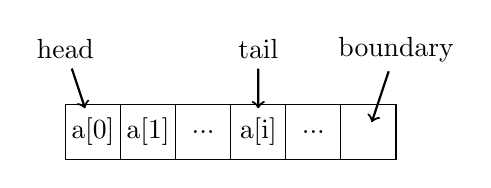
\begin{tikzpicture}[scale=0.7]
    \draw (0, 0) rectangle (1, 1) node (a0) [pos=.5] {a[0]}
          (1, 0) rectangle (2, 1) node [pos=.5] {a[1]}
          (2, 0) rectangle (3, 1) node [pos=.5] {...}
          (3, 0) rectangle (4, 1) node [pos=.5] (ai) {a[i]}
          (4, 0) rectangle (5, 1) node [pos=.5] {...}
          (5, 0) rectangle (6, 1) node (an) [pos=.5] {};
    \draw (0, 2) node (hd) {head}
          (3.5, 2) node (tl) {tail}
          (6, 2) node (bd) {boundary};
    \draw[thick, ->] (hd) edge (a0)
                 (tl) edge (ai)
                 (bd) edge (an);
  \end{tikzpicture}}
 \subcaptionbox{Free cells after dequeue.}{
  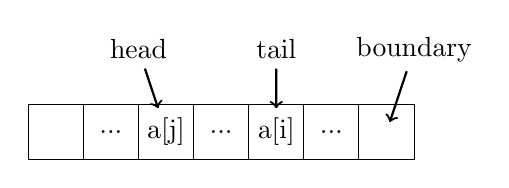
\begin{tikzpicture}[scale=0.7]
    \draw (0, 0) rectangle (1, 1)
          (1, 0) rectangle (2, 1) node [pos=.5] {...}
          (2, 0) rectangle (3, 1) node (aj) [pos=.5] {a[j]}
          (3, 0) rectangle (4, 1) node [pos=.5] {...}
          (4, 0) rectangle (5, 1) node (ai) [pos=.5] {a[i]}
          (5, 0) rectangle (6, 1) node [pos=.5] {...}
          (6, 0) rectangle (7, 1) node (an) [pos=.5] {};
    \draw (2, 2) node (hd) {head}
          (4.5, 2) node (tl) {tail}
          (7, 2) node (bd) {boundary};
    \draw[thick, ->] (hd) edge (aj)
                 (tl) edge (ai)
                 (bd) edge (an);
  \end{tikzpicture}} \\
 \subcaptionbox{Enqueue more elements to the boundary}{
   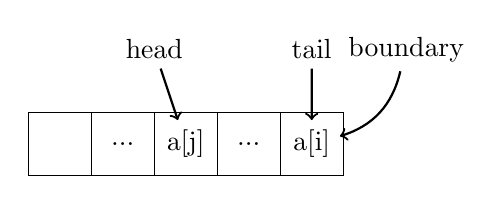
\begin{tikzpicture}[scale=0.8]
    \draw (0, 0) rectangle (1, 1)
          (1, 0) rectangle (2, 1) node [pos=.5] {...}
          (2, 0) rectangle (3, 1) node (aj) [pos=.5] {a[j]}
          (3, 0) rectangle (4, 1) node [pos=.5] {...}
          (4, 0) rectangle (5, 1) node (ai) [pos=.5] {a[i]};
    \draw (2, 2) node (hd) {head}
          (4.5, 2) node (tl) {tail}
          (6, 2) node (bd) {boundary};
    \draw[thick, ->] (hd) edge (aj)
                 (tl) edge (ai)
                 (bd) edge [bend left] (ai);
  \end{tikzpicture}}
 \subcaptionbox{Enqueue the next element to the first cell.}{
    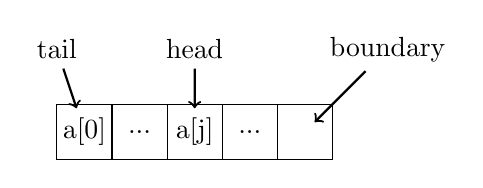
\begin{tikzpicture}[scale=0.7]
    \draw (0, 0) rectangle (1, 1) node (a0) [pos=.5] {a[0]}
          (1, 0) rectangle (2, 1) node [pos=.5] {...}
          (2, 0) rectangle (3, 1) node (aj) [pos=.5] {a[j]}
          (3, 0) rectangle (4, 1) node [pos=.5] {...}
          (4, 0) rectangle (5, 1) node (an) [pos=.5] {};
    \draw (2.5, 2) node (hd) {head}
          (0, 2) node (tl) {tail}
          (6, 2) node (bd) {boundary};
    \draw[thick, ->] (hd) edge (aj)
                 (tl) edge (a0)
                 (bd) edge (an);
  \end{tikzpicture}} \\
 \subcaptionbox{All cells are occupied, full.}{
   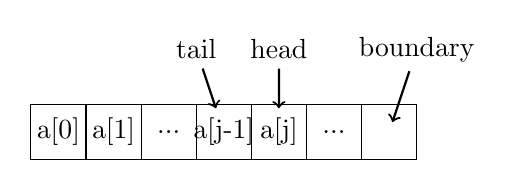
\begin{tikzpicture}[scale=0.7]
    \draw (0, 0) rectangle (1, 1) node [pos=.5] {a[0]}
          (1, 0) rectangle (2, 1) node [pos=.5] {a[1]}
          (2, 0) rectangle (3, 1) node [pos=.5] {...}
          (3, 0) rectangle (4, 1) node (a1j) [pos=.5] {a[j-1]}
          (4, 0) rectangle (5, 1) node (aj) [pos=.5] {a[j]}
          (5, 0) rectangle (6, 1) node [pos=.5] {...}
          (6, 0) rectangle (7, 1) node (an) [pos=.5] {};
    \draw (4.5, 2) node (hd) {head}
          (3, 2) node (tl) {tail}
          (7, 2) node (bd) {boundary};
    \draw[thick, ->] (hd) edge (aj)
                 (tl) edge (a1j)
                 (bd) edge (an);
  \end{tikzpicture}}
 \caption{Circular buffer queue}
 \label{fig:circular-buffer-queue}
\end{figure}

\begin{algorithmic}[1]
\Function{Enqueue}{$Q, x$}
  \If{not \Call{Full}{$Q$}}
    \State \Call{Count}{$Q$} $\gets$ \Call{Count}{$Q$} + 1
    \State tail $\gets $ (\Call{Head}{$Q$} + \Call{Count}{$Q$}) $\bmod$ \Call{Size}{$Q$}
    \State \Call{Buf}{$Q$}[tail] $\gets x$
  \EndIf
\EndFunction
\end{algorithmic}

\begin{algorithmic}[1]
\Function{Dequeue}{$Q$}
  \State $x \gets$ NIL
  \If{not \Call{Empty}{$Q$}}
    \State $h \gets$ \Call{Head}{$Q$}
    \State $x \gets$ \Call{Buf}{$Q$}[$h$]
    \State \Call{Head}{$Q$} $\gets $ (h + 1) $\bmod$ \Call{Size}{$Q$}
    \State \Call{Count}{$Q$} $\gets$ \Call{Count}{$Q$} - 1
  \EndIf
  \State \Return $x$
\EndFunction
\end{algorithmic}

\begin{Exercise}\label{ex:buffered-queue}
\Question{The circular buffer is allocated with a predefined size. We can use two references, head and tail instead. How to determine if a circular buffer queue is full or empty? (the head can be either ahead of tail or behind it.)}
\end{Exercise}

\begin{Answer}[ref = {ex:buffered-queue}]
\Question{The circular buffer is allocated with a predefined size. We can use two references, head and tail instead. How to determine if a circular buffer queue is full or empty? (the head can be either ahead of tail or behind it.)

\vspace{3mm}
Although we can deal with different cases that the head is before/behind the tail, as shown in \cref{fig:circular-buffer-queue}, let us seek for some simple and unified solution. Consider an array with both sides open and are extending infinitely. Let the head index be $h$, the tail be $t$, the size of the buffer be $s$. The range $[h, t)$ (left close, right open) is occupied with elements. The empty/full testing is as below:

\[
\begin{cases}
empty(h, t): & h = t  \\
full(h, t): & t - h = s \\
\end{cases}
\]

The circular buffer is essentially modular arithmetic on top of this. Write $[n]_s = n \bmod s$. Apply to above full test: $[t]_s - [h]_s = [s]_s = 0$, which gives $[t]_s = [h]_s$. It is exactly the empty test condition. It means we can't differentiate empty with full only with the modular result. We need either add a flag (indicate the order between $h$ and $t$), or use the original index (of the infinite long segment) without applying $\bmod$ for the empty/full test. Consider the integer number has limited byte size, we can $\bmod$ the index with a big number $p$ ($p > s$) which is co-prime with $s$:

\[
\begin{cases}
empty(h, t): & [h]_p = [t]_p  \\
full(h, t): & [t - h]_p = s \\
\end{cases}
\]

Below is the example program:

\begin{Bourbaki}
Int P_LIMIT = 104743 // the 10000th prime
Bool empty(Queue<K> q) = (q.h == q.t)
Bool full(Queue<K> q) = (q.s == (q.t - q.h) mod P_LIMIT)

void enqueue(Queue<K> q, K x) {
    if not full(q) {
        q.t = (q.t + 1) mod P_LIMIT
        q.buf[q.t mod q.s] = x
    }
}

Optional<K> dequeue(Queue<K> q) {
    Optional<K> x = Optional.Nothing
    if not empty(q) {
        x = Optional.of(q.buf[q.h mod q.s])
        q.h = (q.h + 1) mod P_LIMIT
    }
    return x
}
\end{Bourbaki}
}
\end{Answer}

\section{Paired-list queue}
\index{Queue!Paired-list queue}

We can access the list head in constant time, but need linear time to access the tail. We connect two lists `tail to tail' to implement queue, as shown in \cref{fig:horseshoe-magnet}. Define the queue as $(f, r)$, where $f$ is the front list, and $r$ is the rear list. The empty list is $([\ ], [\ ])$. We push new element to the head of $r$, and pop from the tail of $f$. Both are constant time.

\begin{figure}[htbp]
  \centering
  \includegraphics[scale=0.6]{img/paired-listq}
  \caption{paired-list queue.}
  \label{fig:horseshoe-magnet}
\end{figure}

\be
\begin{cases}
push\ x\ (f, r) & = (f, x \cons r) \\
pop\ (x \cons f, r)   & = (f, r) \\
\end{cases}
\ee

$f$ may become empty after a series of pops, while $r$ still contains elements. To continue pop, we reverse $r$ to replace $f$, i.e., $([\ ], r) \mapsto (\textit{reverse} r, [\ ])$. We need check and balance in every push/pop:

\be
\begin{array}{rcl}
\textit{balance}\ [\ ]\ r & = & (\textit{reverse}\ r, [\ ]) \\
\textit{balance}\ f\ r & = & (f, r) \\
\end{array}
\ee

Although the time is bound to linear time when reverse $r$, the amortised performance is constant time. Update push/pop as below:

\be
\begin{cases}
push\ x\ (f, r) & = \textit{balance}\ f\ (x \cons r) \\
pop\ (x \cons f, r)   & = \textit{balance}\ f\ r \\
\end{cases}
\ee

\index{Queue!Paired-array queue} \label{sec:paired-array-queue}

There is a symmetric implementation with a pair of arrays (\cref{tab:array-list-comp}). Connect two arrays head to head, as shown in \cref{fig:horseshoe-array}. When $R$ becomes empty, reverse array $F$ to replace $R$.

\begin{table}[htbp]
\centering
\begin{tabular}{l | c | r}
  \hline
  operation & array & list \\
  \hline
  insert to head & $O(n)$ & $O(1)$ \\
  append to tail & $O(1)$ & $O(n)$ \\
  remove from head & $O(n)$ & $O(1)$ \\
  remove from tail & $O(1)$ & $O(n)$ \\
  \hline
\end{tabular}
\caption{array and list}
\label{tab:array-list-comp}
\end{table}

\begin{figure}[htbp]
  \centering
  \includegraphics[scale=0.6]{img/paired-arrayq}
  \caption{paired-array queue.}
  \label{fig:horseshoe-array}
\end{figure}

\begin{Exercise}\label{ex:paired-list-queue}
\Question{Why need balance check and adjustment after push?}
\Question{Do the amortized analysis for the paired-list queue.}
\Question{Implement the paired-array queue.}
\end{Exercise}

\begin{Answer}[ref = {ex:paired-list-queue}]
\Question{Why need balance check and adjustment after push?

Consider the case, first $push\ a\ ([\ ], [\ ])$, then $pop$.
}
\Question{Do the amortized analysis for the paired-list queue.

We use the banker's accounting method. Each element in the rear list $r$ has 1 credit. When push to rear, we take a step to add, and increase 1 credit. The amortized cost is $O(2)$. When pop, if it doesn't cause list reverse, we take a step to remove an element without decreasing the credit. The amortized cost is $O(1)$. If causes list reverse, we take $m$ steps to reverse, and take a step to remove an element, where $m$ is the length of $r$. We also use $m$ credits in $r$. The amortized cost is $O(m + 1 - m) = O(1)$.
}

\Question{Implement the paired-array queue.

\begin{algorithmic}[1]
\Function{Push}{$Q, x$}
  \State \textproc{Append}(\Call{Front}{$Q$}, $x$)
\EndFunction
\Statex
\Function{Pop}{$Q$}
  \If{\Call{Rear}{$Q$} $= [\ ]$}
    \State \Call{Rear}{$Q$} $\gets$ \textproc{Reverse}(\Call{Front}{$Q$})
    \State \Call{Front}{$Q$} $\gets [\ ]$
  \EndIf
  \State $n \gets$ \textproc{Length}(\Call{Rear}{$Q$})
  \State $x \gets$ \Call{Rear}{$Q$}[n]
  \State \textproc{Length}(\Call{Rear}{$Q$}) $\gets n - 1$
  \State \Return $x$
\EndFunction
\end{algorithmic}
}
\end{Answer}

\section{Balance Queue}
\index{Queue!Balance Queue}

Although paired-list queue performs in amortized constant time, it is linear time in worse case. For e.g., there is an element in $f$, then repeat pushing $n$ elements. Now it takes $O(n)$ time to pop. $f$ and $r$ are unbalance in this case. To solve it, we add another rule: the length of $r$ is not greater than $f$, otherwise reverse.

\be
  |r| \leq |f|
\label{eq:balance-invariant}
\ee

We check the lengths in every push/pop, however, it takes linear time to compute length. We can record the length in a variable, and update it during push/pop. Denote the paired-list queue as $(f, n, r, m)$, where $n = |f|$, $m = |r|$. From the balance rule \cref{eq:balance-invariant}, we only need check the length of $f$ to test if a queue is empty:

\be
  Q = \phi \iff n = 0
\ee

Change the definition of push/pop to:

\be
\begin{cases}
  push\ x\ (f, n, r, m) & = \textit{balance}\ (f, n,  x \cons r, m + 1) \\
  pop\ (x \cons f, n, r, m) & = \textit{balance}\ (f, n - 1, r, m) \\
\end{cases}
\ee

Where:

\be
\textit{balance}\ (f, n, r, m) = \begin{cases}
  m \leq n: & (f, n, r, m) \\
  \text{otherwise}: & (f \doubleplus \textit{reverse}\ r, m + n, [\ ], 0)\\
\end{cases}
\ee

\section{Real-time queue}
\index{Queue!Real-time queue} \label{sec:realtime-queue}

It still takes linear time to reverse and concatenate lists in balanced queue. The real-time queue need guarantee constant time in every push/pop operation. The performance bottleneck happens in $f \doubleplus \textit{reverse}\ r$. At this time, $m > n$, breaks the balance rule. Since $m, n$ are integers, we know $m = n + 1$. $\doubleplus$ takes $O(n)$ time, and reverse takes $O(m)$ time. The total time is bound to $O(n + m)$, which is proportion to the number of elements. Our solution is to distribute the computation to multiple push and pop operations. Revisit the tail recursive\cite{wiki-tail-call}\cite{recursion} reverse (in Curried form):

\be
\textit{reverse}\ = \textit{reverse}'\ [\ ]
\ee

where:

\be
\begin{array}{rcl}
\textit{reverse}'\ a\ [\ ] & = & a \\
\textit{reverse}'\ a\ (x \cons xs) & = & \textit{reverse}'\ (x \cons a)\ xs \\
\end{array}
\ee

We turn the tail recursive implementation to stepped computation. Model it as a series of state transformations. Define a state machine with two states: reverse state $S_r$, and complete state $S_f$. We {\em slow-down} the reverse computation as below:

\be
\begin{array}{rcl}
step\ S_r\ a\ [\ ] & = & (S_f, a) \\
step\ S_r\ a\ (x \cons xs) & = & (S_r, (x \cons a), xs) \\
\end{array}
\ee

Each step, we check and transform the state. $S_r$ means the reverse is on going. If there is no remaining element to reverse, we change the state to $S_f$ (done); otherwise, link the head $x$ ahead of $a$. Every step terminates, but not continues running recursively. The new state with the intermediate reverse result is input to the next $step$. For example:

\[
\begin{array}{rcl}
step\ S_r\ \text{``hello''}\ [\ ] & = & (S_r, \text{``ello''}, \text{``h''}) \\
step\ S_r\ \text{``ello''}\ \text{``h''} & = & (S_r, \text{``llo''}, \text{``eh''}) \\
... & & \\
step\ S_r\ \text{``o''}\ \text{``lleh''} & = & (S_r, [\ ], \text{``olleh''}) \\
step\ S_r\ [\ ]\ \text{``olleh''} & = & (S_f, \text{``olleh''})
\end{array}
\]

However, it only solves half problem. We also need slow-down $\doubleplus$ computation, which is more complex. Use state machine again. To concatenate $xs \doubleplus ys$, we first reverse $xs$ to $\overleftarrow{xs}$, then pick elements from $\overleftarrow{xs}$ one by one, and link each ahead of $ys$. The idea is similar to $\textit{reverse}'$:

\be
  \begin{array}{rcl}
    xs \doubleplus ys & = & (\textit{reverse}\ \textit{reverse}\ xs) \doubleplus ys \\
             & = & (\textit{reverse}'\ [\ ]\ \overleftarrow{xs}) \doubleplus ys \\
             & = & \textit{reverse}'\ ys\ \overleftarrow{xs} \\
  \end{array}
\ee

We need add another state: after reverse $r$, step by step concatenate from $\overleftarrow{f}$. The three states are: $S_r$ of reverse, $S_c$ of concatenate, $S_f$ of completion. The two phases are:

\begin{enumerate}
\item Stepped reverse $f$ to $\overleftarrow{f}$, and $r$ to $\overleftarrow{r}$ in parallel;
\item Stepped take elements from $\overleftarrow{f}$, and link each ahead of $\overleftarrow{r}$.
\end{enumerate}

\be
\begin{array}{rcll}
next\ (S_r, f', x \cons f, r', y \cons r) & = & (S_r, x \cons f', f, y \cons r', r) & \text{reverse}\ f, r\\
next\ (S_r, f', [\ ], r', [y]) & = & next\ (S_c, f', y \cons r') & \text{reverse done, start concatenation}\\
next\ (S_c, a, [\ ]) & = & (S_f, a) & \text{done}\\
next\ (S_c, a, x \cons f') & = & (S_c, x \cons a, f') & \text{concatenation}\\
\end{array}
\ee

We need arrange these steps to each push/pop. From the balance rule, when $m = n + 1$, triggers $f \doubleplus \textit{reverse}\ r$. it takes $n + 1$ steps to reverse $r$. Within these steps, we reverse $f$ in parallel. After that, it takes another $n + 1$ steps to concatenate, in total $2n + 2$ steps. The critical question is: Before complete the $2n + 2$ steps, will the queue become unbalanced again due to a series of push/pop operations?

Luckily, repeat pushing won't break the balance rule again before we complete $f \doubleplus \textit{reverse}\ r$. We will obtain a new front list $f' = f \doubleplus \textit{reverse}\ r$ after $2n + 2$ steps, while the time to break the balance rule again is:

\be
  \begin{array}{rcl}
  |r'| & = & |f'| + 1 \\
       & = & |f| + |r| + 1 \\
       & = & 2n + 2
  \end{array}
\ee

Thanks to the balance rule. Even repeat pushing as many as possible, the $2n + 2$ steps are guaranteed to be completed before the next time when the queue is unbalanced, hence the new $f$ will be ready. We can safely start to compute $f' \doubleplus \textit{reverse}\ r'$.

However, pop may happen before the completion of $2n + 2$ steps. We are facing the situation that needs to extract element from $f$, while the new front list $f' = f \doubleplus \textit{reverse}\ r$ hasn't been ready yet. To solve this issue, we duplicate a copy of $f$ when doing $\textit{reverse}\ f$. We are safe even repeat pop for $n$ times. \Cref{tab:pop-before-n} shows the queue during phase 1 (reverse $f$ and $r$ in parallel)\footnote{Although it takes linear time to duplicate a list, however, the one-shot copying won't happen at all. We actually duplicate the reference to the front list, and delay the element level copying to each step}.

\begin{table}[htbp]
\centering
\begin{tabular}{c | c | c}
  $f$ copy & on-going part & new $r$ \\
  \hline
  $\{ f_i, f_{i+1}, ..., f_n \}$ & $(S_r, \tilde{f}, ..., \tilde{r}, ...)$ & $ \{ ... \}$ \\
  first $i-1$ elements out & intermediate $\overleftarrow{f}$, $\overleftarrow{r}$ & newly pushed
\end{tabular}
\caption{Before completion of the first $n$ steps.}
\label{tab:pop-before-n}
\end{table}

The copy of $f$ is exhausted after repeating $n$ pops. We are about to start stepped concatenation. What if pop happens at this time? Since $f$ is exhausted, it becomes $[\ ]$. We needn't concatenate anymore. This is because $f \doubleplus \overleftarrow{r} = [\ ] \doubleplus \overleftarrow{r} = \overleftarrow{r}$. In fact, we only need to concatenate the elements in $f$ that haven't been popped. Because we pop from the head of $f$, let us use a counter to record the remaining elements in $f$. It's initialized as 0. We apply +1 every time when reverse an element. It means we need concatenate this element in the future; Whenever pop happens, we apply -1, means we needn't concatenate this one any more. We also decrease it during concatenation, and cancel the process when it is 0. Below is the updated state transformation:

\be
\begin{array}{rcll}
next\ (S_r, n, f', x \cons f, r', y \cons r) & = & (S_r, n + 1, x \cons f', f, y \cons r', r) & \text{reverse}\ f, r\\
next\ (S_r, n, f', [\ ], r', [y]) & = & next\ (S_c, n, f', y \cons r') & \text{reverse done, start concatenation}\\
next\ (S_c, 0, a, f) & = & (S_f, a) & \text{done}\\
next\ (S_c, n, a, x \cons f') & = & (S_c, n - 1, x \cons a, f') & \text{concatenation}\\
next\ S_0 & = & S_0 & \text{idle} \\
\end{array}
\ee

We define an addition idle state $S_0$ to simplify the logic. The queue contains 3 parts: the front list $f$ with its length $n$, the state $S$ of on-going $f \doubleplus \textit{reverse}\ r$, and the rear list $r$ with its length $m$. Denoted as $(f, n, S, r, m)$. The empty queue is $([\ ], 0, S_0, [\ ], 0)$. The queue is empty when $n = 0$ according to the balance rule. Update the push/pop as:

\be
\begin{cases}
  push\ x\ (f, n, S, r, m) & = balance\ f\ n\ S\ (x \cons r)\ (m + 1) \\
  pop\ (x \cons f, n, S, r, m) & = balance\ f\ (n - 1)\ (abort\ S)\ r\ m \\
\end{cases}
\ee

Where $abort$ decreases the counter to cancel an element for concatenation. We'll define it later. $balance$ triggers stepped $f \doubleplus \textit{reverse}\ r$ if the queue is unbalanced, otherwise runs a step:

\be
balance\ f\ n\ S\ r\ m = \begin{cases}
  m \leq n: & step\ f\ n\ S\ r\ m \\
  \text{otherwise}: & step\ f\ (n + m)\ (next\ (S_r, 0, [\ ], f, [\ ], r))\ [\ ]\ 0 \\
\end{cases}
\ee

Where $step$ transforms the state machine, ends with the idle state $S_0$ when completes.

\be
step\ f\ n\ S\ r\ m = queue\ (next\ S)
\ee

Where:

\be
\begin{array}{rcll}
queue\ (S_f, f') & = & (f', n, S_0, r, m) & \text{replace $f$ with $f'$} \\
queue\ S' & = & (f, n, S', r, m) & \\
\end{array}
\ee

Finally, define $abort$ to cancel an element:

\be
\begin{array}{rcl}
abort\ (S_c, 0, (x \cons a), f') & = & (S_f, a) \\
abort\ (S_c, n, a, f') & = & (S_c, n - 1, a, f') \\
abort\ (S_r, n, f' f, r' r) & = & (S_r, n - 1, f', f, r', r) \\
abort\ S & = & S
\end{array}
\ee

\begin{Exercise}\label{ex:realtime-queue}
\Question{Why need rollback an element (we cancelled the previous `cons', removed $x$ and return $a$ as the result) when $n=0$ in $abort$? }
\Question{Implement the real-time queue with paired arrays. We can't copy the array when start rotation, or the performance will downgrade to linear time. Please implement `lazy' copy, i.e., copy an element per step.}
\end{Exercise}

\begin{Answer}[ref = {ex:realtime-queue}]
\Question{Why need rollback an element (we cancelled the previous `cons', removed $x$ and return $a$ as the result) when $n=0$ in $abort$?

The $abort$ function is only called during pop. When $n = 0$, the rotate just finished, it is about to transform the state from $(S_c, 0, (x \cons a), f')$ to $(S_f, a)$. While $x$ being linked previously is the one to be popped, hence, we need remove $x$ and return $a$ as the result.
}

\Question{Implement the real-time queue with paired arrays. We can't copy the array when start rotation, or the performance will downgrade to linear time. Please implement `lazy' copy, i.e., copy an element per step.

Assume we can get the length of an array in constant time. We push element to the tail of array $f$, and pop from the tail of array $r$. When the two arrays are not balanced, start a state machine to compute $acc = reverse(f) \doubleplus r$ step by step. If $f \neq [\ ]$, we extract the tail element and append to the tail of $acc$. After reversed $f$, we copy the elements from the left of $r$, and append to the tail of $acc$ one by one, i.e., $append(acc, r[i])$, where $i = 0, 1, .., |r| - 1$. While rotating in steps, one can still pop from the tail of $r$, the rotation completes when $i$ exceeds $|r|$.

\begin{Bourbaki}
data State<K> {
    [K] acc, front, rear
    Int idx

    State([K] f, [K] r) {
        acc = [], front = f, rear = r
        idx = 0
    }

    // compute reverse(f) ++ r step by step
    Self step() {
        if front != [] then acc.append(front.popLast())  // reversing
        if s.front == [] and idx < length(rear) {    // concatenating
            acc.append(rear[idx])
            idx = idx + 1
        }
    }

    Bool done() = (front == [] and length(rear) < idx)
}

data RealtimeQueue<K> {
    [K] front = []
    [K] rear = []
    State<K> state = null

    Bool isEmpty() = (front == [] and rear == [])

    Self push(K x) {
        front.append(x)
        balance()
    }

    K pop() {
        x = rear.popLast()
        balance()
        return x
    }

    Void balance() {
        if state == null and length(rear) < length(front) {
            state = State(front, rear).step()
            front = []
        }
        if state != null and state.step().done() {
            rear = state.acc
            state = null
        }
    }
}
\end{Bourbaki}
}
\end{Answer}

\section{Lazy real-time queue}
\index{Queue!Lazy real-time queue}

The key to realize real-time queue is to break down the expensive
$f \doubleplus \textit{reverse}\ r$. We can simplify it with lazy evaluation. Assume function \textit{rotate} computes $f \doubleplus \textit{reverse}\ r$ in steps, i.e., below two functions are equivalent with an accumulator $a$.
\be
  \textit{rotate}\ xs\ ys\ a = xs \doubleplus (\textit{reverse}\ ys) \doubleplus a
  \label{eq:rot-def}
\ee

Initialize $xs$ as the front list $f$, $ys$ as the rear list $r$,
the accumulator $a$ empty $[\ ]$. We implement \textit{rotate} from the edge case:

\be
  \textit{rotate}\ [\ ]\ [y]\ a = y \cons a
\ee

The recursive case is:

\be
  \begin{array}{cll}
  & \textit{rotate}\ (x \cons xs)\ (y \cons ys)\ a & \\
  = & (x \cons xs) \doubleplus (\textit{reverse}\ (y \cons ys)) \doubleplus a & \text{from \cref{eq:rot-def}} \\
  = & x : (xs \doubleplus \textit{reverse}\ (y \cons ys)) \doubleplus a) & \text{concatenation is associative} \\
  = &  x : (xs \doubleplus \textit{reverse}\ ys \doubleplus (y \cons a)) & \text{reverse property, and associative} \\
  = & x : \textit{rotate}\ xs\ ys\ (y \cons a) & \text{reverse of \cref{eq:rot-def}}
  \end{array}
\ee

Summarize together:

\be
\begin{array}{rcl}
\textit{rotate}\ [\ ]\ [y]\ a & = & y \cons a \\
\textit{rotate}\ (x \cons xs)\ (y \cons ys)\ a & = & x : \textit{rotate}\ xs\ ys\ (y \cons a) \\
\end{array}
\ee

In lazy evaluation settings, (:) is delayed to push/pop, hence the \textit{rotate} is broken down. We change the paired-list queue definition to $(f, r, rot)$, where $rot$ is the on-going $f \doubleplus \textit{reverse}\ r$ computation. It is initialized empty $[\ ]$.

\be
\begin{cases}
push\ x\ (f, r, rot) & = balance\ f\ (x \cons r)\ rot \\
pop\ (x \cons f, r, rot) & = balance\ f\ r\ rot \\
\end{cases}
\ee

Every time, $balance$ advances the rotation one step, and starts another round when completes.

\be
\begin{array}{rcll}
balance\ f\ r\ [\ ] & = & (f', [\ ], f') & \text{where}: f' = rotate\ f\ r\ [\ ] \\
balance\ f\ r\ (x \cons rot) & = & (f, r, rot) & \text{advance the rotation}\\
\end{array}
\ee

\begin{Exercise}
Implement bidirectional queue, support add/remove elements on both head and tail in constant time.
\end{Exercise}

\section{Appendix - example programs}

List implemented queue:

\begin{lstlisting}[language = Bourbaki]
Queue<K> enQ(Queue<K> q, K x) {
    var p = Node(x)
    p.next = null
    q.tail.next = p
    q.tail = p
    return q
}

K deQ(Queue<K> q) {
    var p = q.head.next   //the next of S
    q.head.next = p.next
    if q.tail == p then q.tail = q.head //empty
    return p.key
}
\end{lstlisting}

Circular buffer queue:

\begin{lstlisting}[language = Bourbaki]
data Queue<K> {
    [K] buf
    int head, cnt, size

    Queue(int max) {
        buf = Array<K>(max)
        size = max
        head = cnt = 0
    }
}
\end{lstlisting}

Enqueue, dequeue implementation for circular buffer queue:

\begin{lstlisting}
N offset(N i, N size) = if i < size then i else i - size

void enQ(Queue<K> q, K x) {
    if q.cnt < q.size {
        q.buf[offset(q.head + q.cnt, q.size)] = x;
        q.cnt = q.cnt + 1
    }
}

K head(Queue<K> q) = if q.cnt == 0 then null else q.buf[q.head]

K deQ(Queue<K> q) {
    K x = null
    if q.cnt > 0 {
        x = head(q)
        q.head = offset(q->head + 1, q->size);
        q.cnt = q.cnt -1
    }
    return x
}
\end{lstlisting}

Real-time queue:

\begin{Haskell}
data State a = Empty
             | Reverse Int [a] [a] [a] [a] -- n, acc f, f, acc r, r
             | Concat Int [a] [a]          -- n, acc, reversed f
             | Done [a]  -- f' = f ++ reverse r

-- f, n = length f, state, r, m = length r
data RealtimeQueue a = RTQ [a] Int (State a) [a] Int

push x (RTQ f n s r m) = balance f n s (x:r) (m + 1)

pop (RTQ (_:f) n s r m) = balance f (n - 1) (abort s) r m

top (RTQ (x:_) _ _ _ _) = x

balance f n s r m
    | m <= n =  step f n s r m
    | otherwise = step f (m + n) (next (Reverse 0 [] f [] r)) [] 0

step f n s r m = queue (next s) where
  queue (Done f') = RTQ f' n Empty r m
  queue s' = RTQ f n s' r m

next (Reverse n f' (x:f) r' (y:r)) = Reverse (n + 1) (x:f') f (y:r') r
next (Reverse n f' [] r' [y]) = next $ Concat n (y:r') f'
next (Concat 0 acc _) = Done acc
next (Concat n acc (x:f')) = Concat (n-1) (x:acc) f'
next s = s

abort (Concat 0 (_:acc) _) = Done acc -- rollback 1 elem
abort (Concat n acc f') = Concat (n - 1) acc f'
abort (Reverse n f' f r' r) = Reverse (n - 1) f' f r' r
abort s = s
\end{Haskell}

Lazy real-time queue:

\begin{Haskell}
data LazyRTQueue a = LQ [a] [a] [a] -- front, rear, f ++ reverse r

empty = LQ [] [] []

push (LQ f r rot) x = balance f (x:r) rot

pop (LQ (_:f) r rot) = balance f r rot

top (LQ (x:_) _ _) = x

balance f r [] = let f' = rotate f r [] in LQ f' [] f'
balance f r (_:rot) = LQ f r rot

rotate [] [y] acc = y:acc
rotate (x:xs) (y:ys) acc = x : rotate xs ys (y:acc)
\end{Haskell}

\ifx\wholebook\relax \else
\section{Answers}
\shipoutAnswer

\begin{thebibliography}{99}

\bibitem{PODC96}
Maged M. Michael and Michael L. Scott. ``Simple, Fast, and Practical Non-Blocking and Blocking Concurrent Queue Algorithms''. \url{http://www.cs.rochester.edu/research/synchronization/pseudocode/queues.html}

\bibitem{SutterDDJ}
Herb Sutter. ``Writing a Generalized Concurrent Queue''. Dr. Dobb's Oct 29, 2008. \url{http://drdobbs.com/cpp/211601363?pgno=1}

\bibitem{CLRS}
Thomas H. Cormen, Charles E. Leiserson, Ronald L. Rivest and Clifford Stein. ``Introduction to Algorithms, Second Edition''. The MIT Press, 2001. ISBN: 0262032937.

\bibitem{okasaki-book}
Chris Okasaki. ``Purely Functional Data Structures''. Cambridge university press, (July 1, 1999), ISBN-13: 978-0521663502

\bibitem{tail-call}
Wikipedia. ``Tail-call''. \url{https://en.wikipedia.org/wiki/Tail_call}

\bibitem{recursion}
Wikipedia. ``Recursion (computer science)''. \url{https://en.wikipedia.org/wiki/Recursion_(computer_science)#Tail-recursive_functions}

\bibitem{SICP}
Harold Abelson, Gerald Jay Sussman, Julie Sussman. ``Structure and Interpretation of Computer Programs, 2nd Edition''. MIT Press, 1996, ISBN 0-262-51087-1

\end{thebibliography}

\expandafter\enddocument
\fi
